
\subsection{Robustness to query scale}
\label{app:query}
In Figure~\ref{fig:query_scale}, we show that the trained model is quite robust to scaling the query input (while keeping the in-context examples fixed): the error does not increase much as we scale up the query
input by a factor of up to 2, or scale down by a factor of up to 16, and degrades slowly after that.

\begin{figure}[htp]
        \centering
        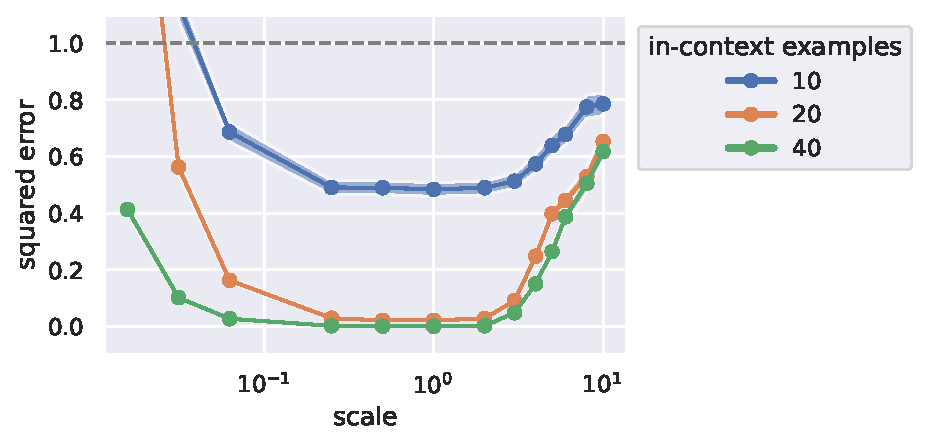
\includegraphics[width=.6\textwidth]{figures/scale_transformer.pdf}
    \caption{\emph{Robustness to the scale of query input.} For a fixed set of in-context examples, we measure the model's error as we scale the query input by a scalar.}
    \label{fig:query_scale}
\end{figure}

\clearpage
\subsection{Out-of-distribution prompts}
\label{app:dist_shift}
Here, we describe the structure of our out-of-distribution prompts (cf.\  Section~\ref{sec:distribution_shifts}), and show the corresponding plots (Figure~\ref{fig:ood_prompts}). 
To avoid conflating factors, we normalize the prompt inputs such that their expected norm is equal to the expected norm of inputs during training and investigate the role of scaling these inputs separately.
We summarize how these prompts deviate from those seen during training in the table below.
\begin{center}
    \begin{tabular}{lccc}
    \toprule
        Prompting strategy
        & $D_\mathcal{X}^{\text{train}} \neq D_\mathcal{X}^{\text{test}}$
        & $D_\mathcal{F}^{\text{train}} \neq D_\mathcal{F}^{\text{test}}$
        & $D_{\text{query}}^\text{test} \neq D_\mathcal{X}^{\text{test}}$ \\
    \midrule
        Skewed covariance & \checkmark \\
        $d/2$-dimensional subspace  & \checkmark \\
        Scale inputs & \checkmark \\
    \midrule
        Noisy output &  & \checkmark \\
        Scale weights & & \checkmark \\
    \midrule
        Different Orthants & \checkmark & & \checkmark \\
        Orthogonal query & & & \checkmark \\
        Query matches example & & & \checkmark \\
    \bottomrule
    \end{tabular}
\end{center}


\paragraph{Skewed covariance.} (Figure \ref{fig:skewed_app}) We sample inputs from $N(0, \Sigma)$ where $\Sigma$ is a skewed covariance matrix with eigenbasis chosen uniformly at random and $i^{\text{th}}$ eigenvalue proportional to $\nicefrac{1}{i^2}$.

\paragraph{Low-dimensional subspace.} (Figure \ref{fig:half_app}) We sample prompt inputs from a random $d/2$ dimensional subspace. That is, we pick a random $d/2$ dimensional subspace, and draw the prompt inputs from an isotropic Gaussian distribution restricted to this subspace.
As a result, it is possible to achieve zero error after $d/2$ in-context examples.

\paragraph{Prompt scale.} (Figure \ref{fig:scale_app}) We consider the setting where the prompt scale between training and inference is different. We either scale the prompt inputs or the weight vectors, by a factor $\{1/3, 1/2,  2, 3\}$.

\paragraph{Noisy linear regression.} (Figure \ref{fig:noisy_app}) We add noise to each prompt output, that is, the $i^{\text{th}}$ output is equal to $w^T x_i + \epsilon_i$ where $\epsilon_i \sim N(0, d/20)$. 

\paragraph{Different orthants for in-context and query inputs.}(Figure \ref{fig:random_app}) We fix the sign of each coordinate to be positive or negative for all in-context inputs $x_i$ (at random), and draw $x_\text{query}$ (as before) i.i.d. from $N(0, I_d)$. 
As a result, all in-context inputs lie in the same orthant, while the query input lies in another orthant with high probability.

\paragraph{Query input orthogonal to in-context inputs.}(Figure \ref{fig:orthogonal_app}) We choose the query input randomly in the space orthogonal to the space spanned by in-context example inputs.
That is, we  draw the query input from an isotropic Gaussian distribution restricted to the subspace orthogonal to the space spanned by the in-context examples. 
Thus, the optimal normalized error is 1 for any number of in-context examples (there can be at most $d-1$ in-context examples for an orthogonal query to exist).

\paragraph{Query input matches an in-context example.}(Figure \ref{fig:overlapping_app})
We set the query input equal to one of the in-context examples chosen uniformly at random.
Thus it's possible to achieve zero error since the in-context examples include the correct prediction for the query input already.


\begin{figure}[htp]
    \begin{subfigure}[b]{0.33\textwidth}
        \centering
        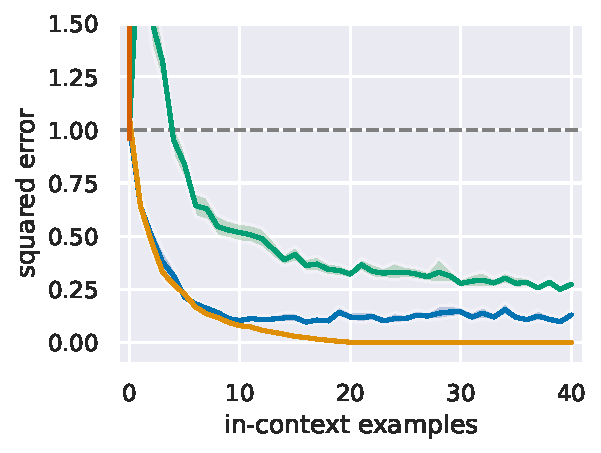
\includegraphics[height=.75\textwidth]{figures/skewed.pdf}
        \caption{skewed covariance}
        \label{fig:skewed_app}
    \end{subfigure} 
    \begin{subfigure}[b]{0.33\textwidth}
        \centering
        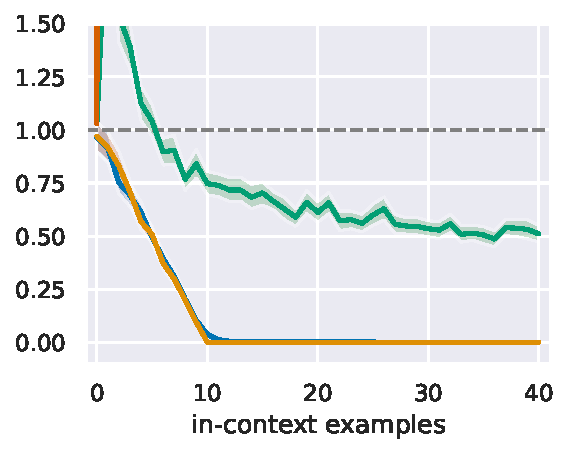
\includegraphics[height=.75\textwidth]{figures/half.pdf}
        \caption{$d$/2-dimensional subspace}
        \label{fig:half_app}
    \end{subfigure}  
    \begin{subfigure}[b]{0.33\textwidth}
        \centering
        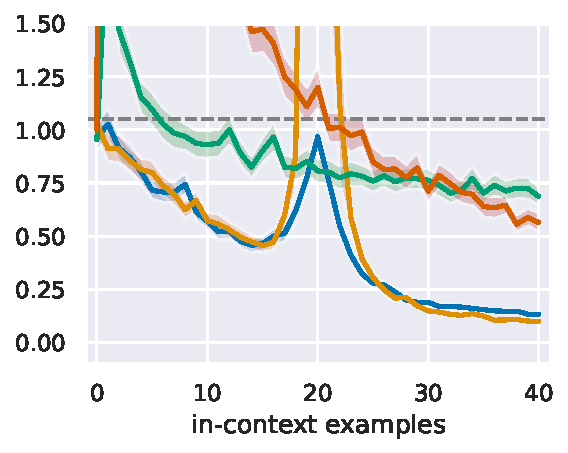
\includegraphics[height=.75\textwidth]{figures/noisyLR.pdf}
        \caption{noisy output}
        \label{fig:noisy_app}
    \end{subfigure} \\[.4em]
    
    \begin{subfigure}[b]{0.33\textwidth}
        \centering
        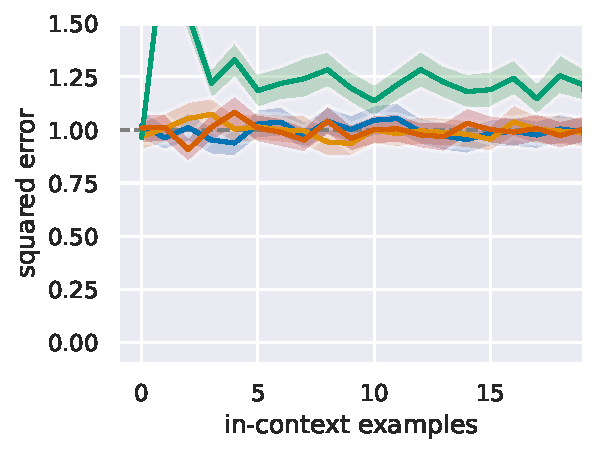
\includegraphics[height=.75\textwidth]{figures/orthogonal.pdf}
        \caption{orthogonal query}
        \label{fig:orthogonal_app}
    \end{subfigure}
    \begin{subfigure}[b]{0.33\textwidth}
        \centering
        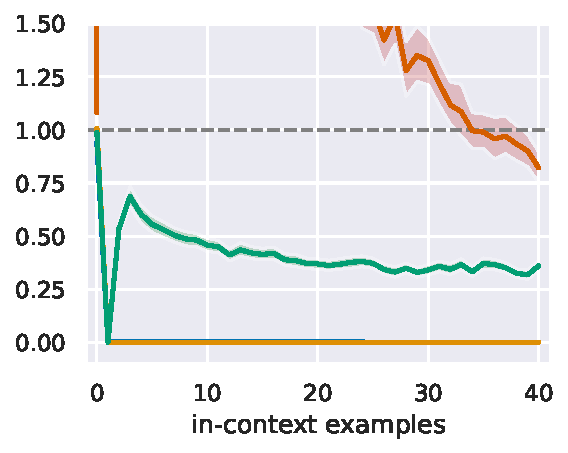
\includegraphics[height=.75\textwidth]{figures/overlapping.pdf}
        \caption{query matches in-context example}
        \label{fig:overlapping_app}
    \end{subfigure}
        \begin{subfigure}[b]{0.33\textwidth}
        \centering
        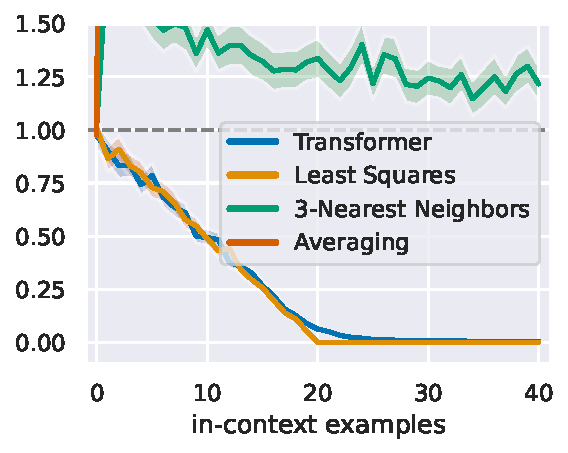
\includegraphics[height=.75\textwidth]{figures/random.pdf}
        \caption{different orthants}
        \label{fig:random_app}
    \end{subfigure}
    \caption{\emph{In-context learning on out-of-distribution prompts.}
    We evaluate the model trained to in-context learn linear functions on prompt distribution  that deviates from the training prompt distribution. 
    In general, the model error degrades gracefully and closely tracks that of the least squares estimator.
    }
    \label{fig:ood_prompts}
\end{figure}

\begin{figure}[htp]
\centering
    \begin{subfigure}[b]{0.42\textwidth}
        \centering
        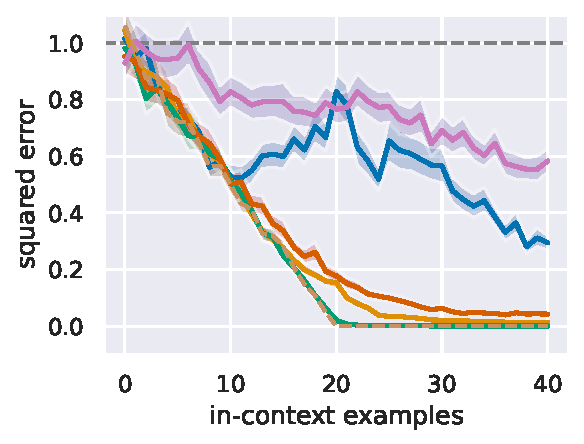
\includegraphics[height=.7\textwidth]{figures/scalex_transformer.pdf}
        \caption{scaled $x$, Transformer}
        \label{fig:scalex_transformer_app}
    \end{subfigure}
    \begin{subfigure}[b]{0.42\textwidth}
        \centering
        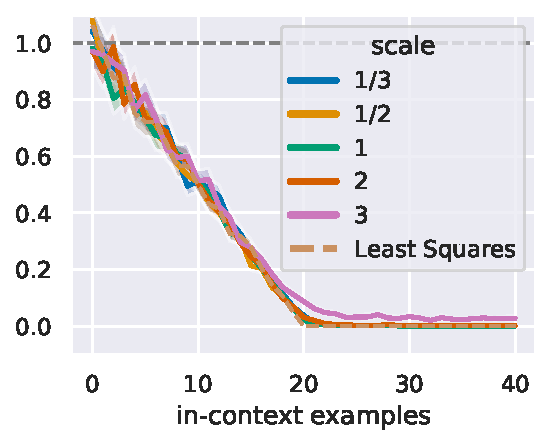
\includegraphics[height=.7\textwidth]{figures/scaley_transformer.pdf}
        \caption{scaled $w$, Transfomer}
        \label{fig:scaley_transformer_app}
    \end{subfigure}
    \caption{\emph{In-context learning robustness to prompt scaling.}
    We evaluate the model trained to in-context learn linear functions when we scaled the prompt inputs $x$ or the weight of the function class $w$. 
    The model appear to be quite robust to scaling $w$ but their performance degrades when scaling the inputs up or down by a factor of 3.}
    \label{fig:scale_app}
\end{figure}


\clearpage
\subsection{Effect of problem dimension and model capacity}
\label{app:capacity}
We plot the model error for additional out-of-distribution prompts in Figure~\ref{fig:capacity_app} for $2d$ in-context examples (with the exception of orthogonal queries where we use $d-1$ in-context examples). 

Similar to the settings in Section \ref{sec:factors} (skewed covariance and different orthants), accuracy improves with capacity in most cases. One exception is scaling $x$ (Figure \ref{fig:capacity_scale_x_2}), in which case we do not see any clear trend. In the case of noisy output (Figure \ref{fig:capacity_noisy}), the accuracy almost saturates at 1.2M parameters, close to the error of the least squares estimator.
In the case of orthogonal query input (Figure \ref{fig:capacity_orthogonal}), the model achieves the optimum error of $1$ even with the tiny model with 0.2M parameters.


\begin{figure}[htp]
    \centering
    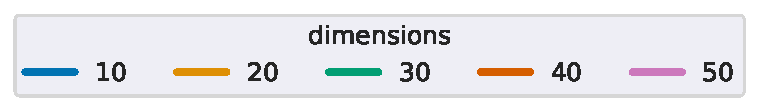
\includegraphics[width=.4\textwidth]{figures/capacity_legend.pdf}
    
    \centering
    \begin{subfigure}[b]{0.325\textwidth}
        \centering
        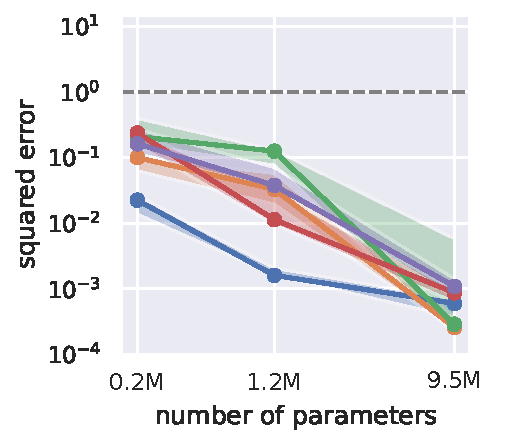
\includegraphics[height=.8\textwidth]{figures/capacity_half.pdf}
        \caption{$d/2$-dimensional subspace}
        \label{fig:capacity_half}
    \end{subfigure} 
    \begin{subfigure}[b]{0.325\textwidth}
        \centering
        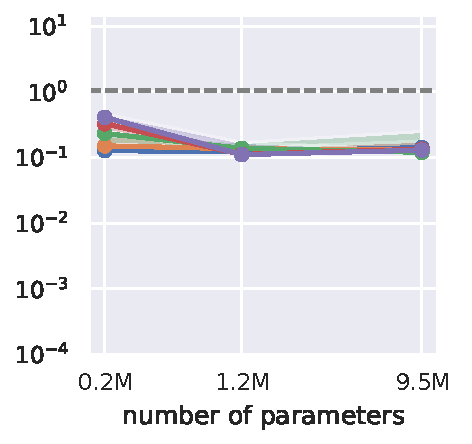
\includegraphics[height=.8\textwidth]{figures/capacity_noisyLR.pdf}
        \caption{noisy output}
        \label{fig:capacity_noisy}
    \end{subfigure} 
    \begin{subfigure}[b]{0.325\textwidth}
        \centering
        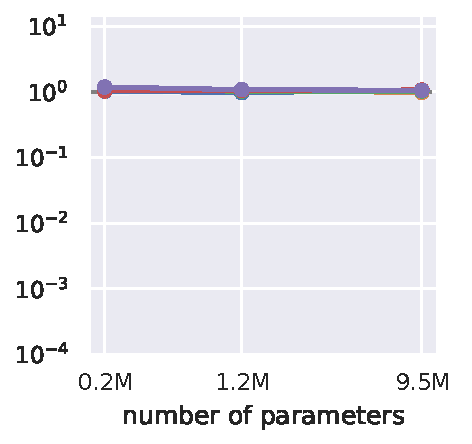
\includegraphics[height=.8\textwidth]{figures/capacity_orthogonal.pdf}
        \caption{orthogonal query}
        \label{fig:capacity_orthogonal}
    \end{subfigure}
    
    \centering
    \begin{subfigure}[b]{0.325\textwidth}
        \centering
        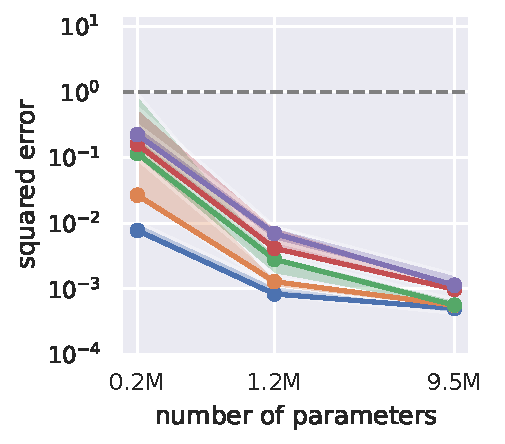
\includegraphics[height=.8\textwidth]{figures/capacity_overlapping.pdf}
        \caption{query matches in-context examples}
        \label{fig:capacity_overlapping}
    \end{subfigure}
    \begin{subfigure}[b]{0.325\textwidth}
        \centering
        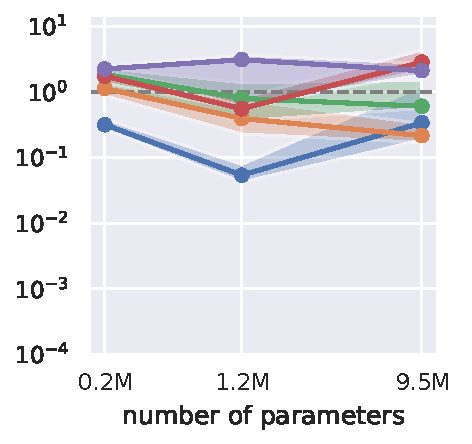
\includegraphics[height=.8\textwidth]{figures/capacity_scale-x=2.pdf}
        \caption{scale $x$ by a factor of 2}
        \label{fig:capacity_scale_x_2}
    \end{subfigure}
    \begin{subfigure}[b]{0.325\textwidth}
        \centering
        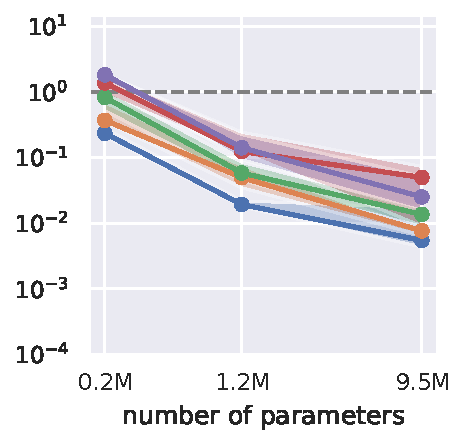
\includegraphics[height=.8\textwidth]{figures/capacity_scale-y=2.pdf}
        \caption{scale $w$ by a factor of 2}
        \label{fig:capacity_scale_y_2}
    \end{subfigure}
    \hfill
    \phantom{}
      \caption{\emph{The effect of model capacity and problem dimension for in-context learning performance on out-of-distribution prompts.} We train Transformer models of varying capacity to in-context learn linear function in varying dimensions $d$. We plot the error with $2d$ in-context examples (or $d-1$ for orthogonal queries). We find that capacity helps in most cases, with the exception of scaling $x$ where we find no clear trend. For each setting, we train 3 models with different random seeds, and show the median error (solid lines), and the minimum and maximum errors (shaded region). (See Figures~\ref{fig:cap_random},~ \ref{fig:cap_skewed} in the main text for the corresponding plots on different-orthants and skewed-covariance.)}
    \label{fig:capacity_app}
\end{figure}

\clearpage
\subsection{Training variance}
\label{app:variance}
In Figure~\ref{fig:trials}, we show the variance in error across training runs for the standard Transformer model (9.5M parameters). We plot the squared error for 3 models (with different random seeds) each for $d \in\{10, 20, 30, 40, 50\} $, trained to in-context learn linear functions.
The error is quite concentrated in the standard setting as well as for most out-of-distribution prompts. In the different-orthants and skewed-covariance settings, we observe a high variance for higher dimensional problems $(d \geq 30)$. However, in Section \ref{sec:factors}, we saw that the error in these settings usually decreases as we increase the model size. 
%If this behaviour continues as we further increase the model size, we would expect to get error concentrated around $0$ (given enough in-context examples) in these settings as well. 
In the setting where we scale $x$, there is high variance even when $d=10$.

\begin{figure}[htp]
    \begin{subfigure}[b]{\textwidth}
        \centering
        
\includegraphics[width=.8\textwidth]{figures/trials/trial_legend.pdf}
        
        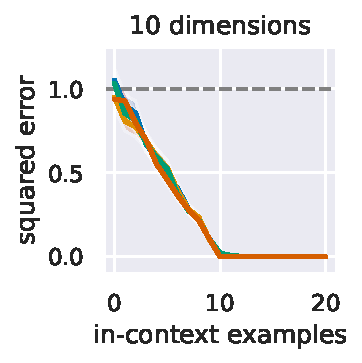
\includegraphics[height=.18\textwidth]{figures/trials/trial_standard_10.pdf}
        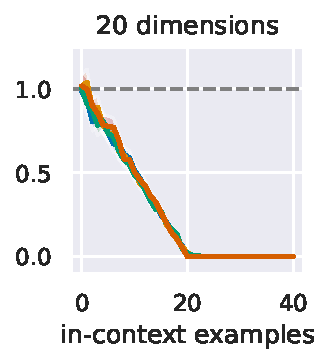
\includegraphics[height=.18\textwidth]{figures/trials/trial_standard_20.pdf}
        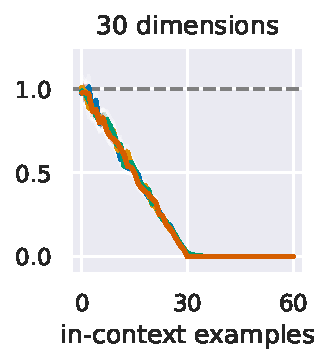
\includegraphics[height=.18\textwidth]{figures/trials/trial_standard_30.pdf}
        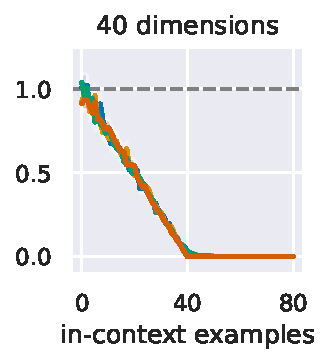
\includegraphics[height=.18\textwidth]{figures/trials/trial_standard_40.pdf}
        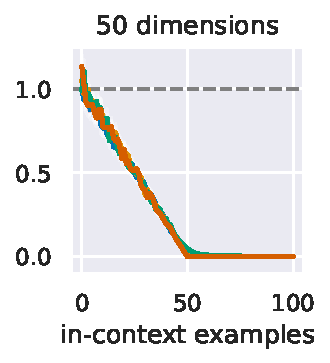
\includegraphics[height=.18\textwidth]{figures/trials/trial_standard_50.pdf}
        \caption{standard}
        \label{fig:trial_standard}
    \end{subfigure} \\[.6em]
    \begin{subfigure}[b]{\textwidth}
        \centering
        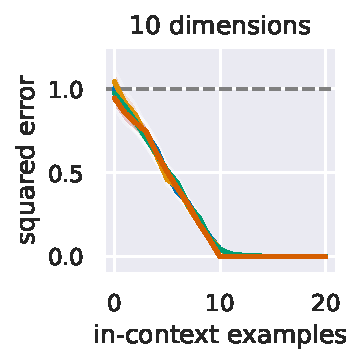
\includegraphics[height=.18\textwidth]{figures/trials/trial_random_10.pdf}
        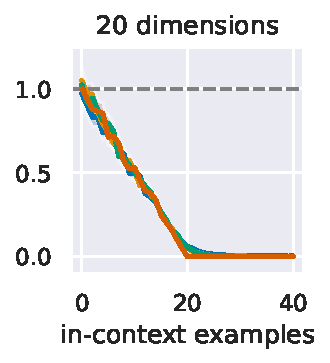
\includegraphics[height=.18\textwidth]{figures/trials/trial_random_20.pdf}
        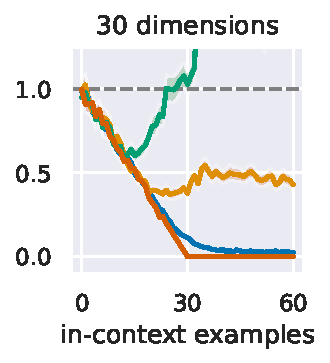
\includegraphics[height=.18\textwidth]{figures/trials/trial_random_30.pdf}
        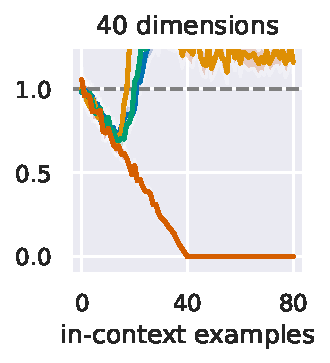
\includegraphics[height=.18\textwidth]{figures/trials/trial_random_40.pdf}
        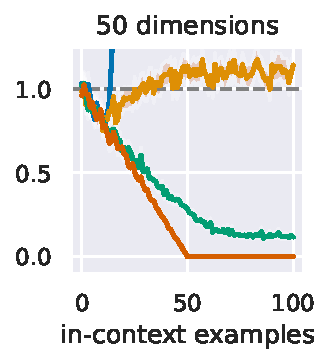
\includegraphics[height=.18\textwidth]{figures/trials/trial_random_50.pdf}
        \caption{different orthants}
        \label{fig:trial_random}
    \end{subfigure} \\[.6em]
    \begin{subfigure}[b]{\textwidth}
        \centering
        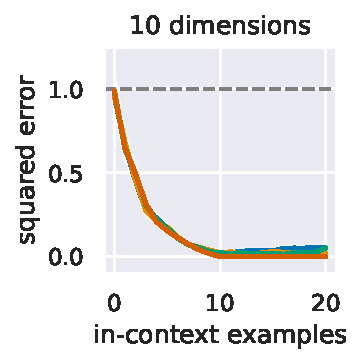
\includegraphics[height=.18\textwidth]{figures/trials/trial_skewed_10.pdf}
        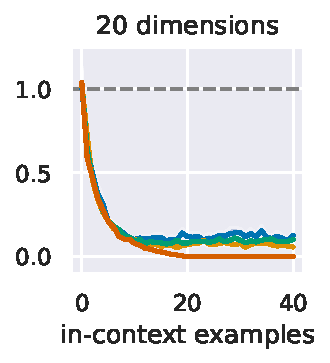
\includegraphics[height=.18\textwidth]{figures/trials/trial_skewed_20.pdf}
        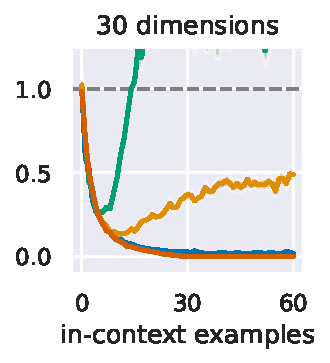
\includegraphics[height=.18\textwidth]{figures/trials/trial_skewed_30.pdf}
        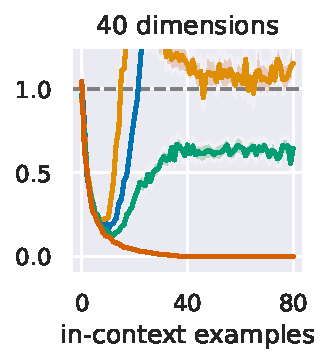
\includegraphics[height=.18\textwidth]{figures/trials/trial_skewed_40.pdf}
        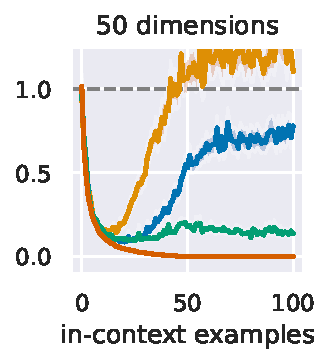
\includegraphics[height=.18\textwidth]{figures/trials/trial_skewed_50.pdf}
        \caption{skewed covariance}
        \label{fig:trial_skewed}
    \end{subfigure} \\[.6em]
    \begin{subfigure}[b]{\textwidth}
        \centering
        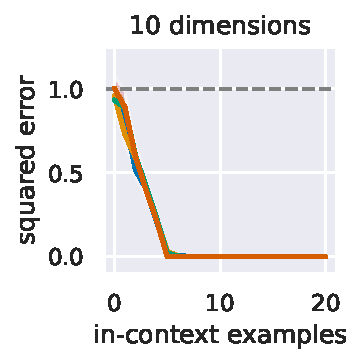
\includegraphics[height=.18\textwidth]{figures/trials/trial_half_10.pdf}
        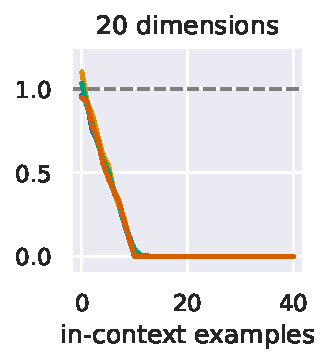
\includegraphics[height=.18\textwidth]{figures/trials/trial_half_20.pdf}
        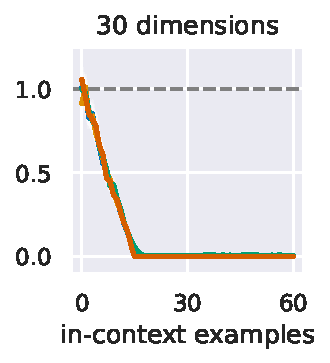
\includegraphics[height=.18\textwidth]{figures/trials/trial_half_30.pdf}
        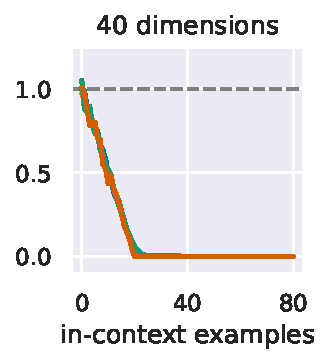
\includegraphics[height=.18\textwidth]{figures/trials/trial_half_40.pdf}
        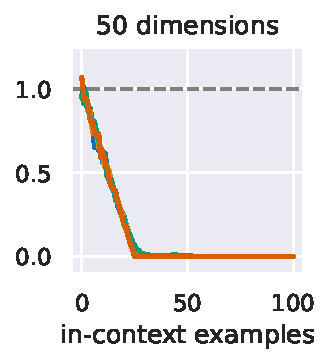
\includegraphics[height=.18\textwidth]{figures/trials/trial_half_50.pdf}
        \caption{$d/2$-dimensional subspace}
        \label{fig:trial_half}
    \end{subfigure}
    % \caption{}
    \caption{\emph{Errors for models trained with different random seeds.} For each dimension, we train three models with different random seeds and show the corresponding error curves.}
    \end{figure}
    \begin{figure}[htp]\ContinuedFloat
    \begin{subfigure}[b]{\textwidth}
        \centering
        
\includegraphics[width=.8\textwidth]{figures/trials/trial_legend.pdf}
        
        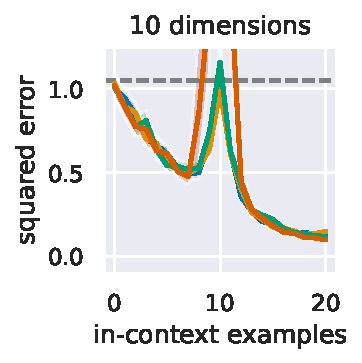
\includegraphics[height=.18\textwidth]{figures/trials/trial_noisyLR_10.pdf}
        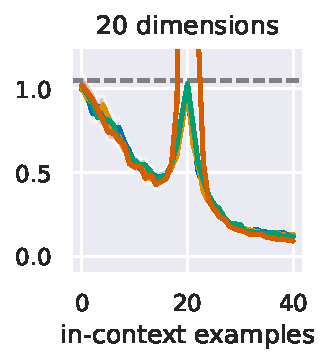
\includegraphics[height=.18\textwidth]{figures/trials/trial_noisyLR_20.pdf}
        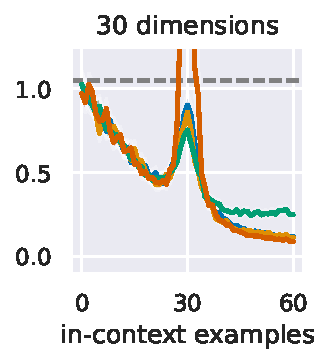
\includegraphics[height=.18\textwidth]{figures/trials/trial_noisyLR_30.pdf}
        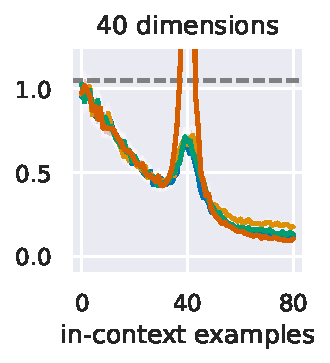
\includegraphics[height=.18\textwidth]{figures/trials/trial_noisyLR_40.pdf}
        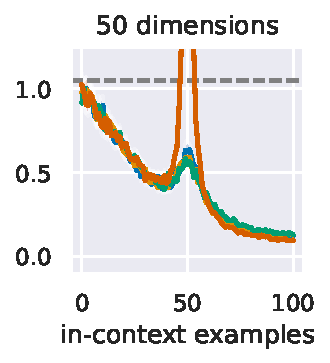
\includegraphics[height=.18\textwidth]{figures/trials/trial_noisyLR_50.pdf}
        \caption{noisy output}
        \label{fig:trial_noisy}
    \end{subfigure} \\[.7em]
    \begin{subfigure}[b]{\textwidth}
        \centering
        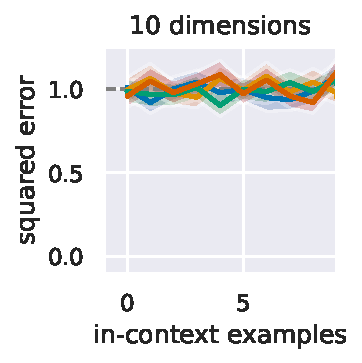
\includegraphics[height=.18\textwidth]{figures/trials/trial_orthogonal_10.pdf}
        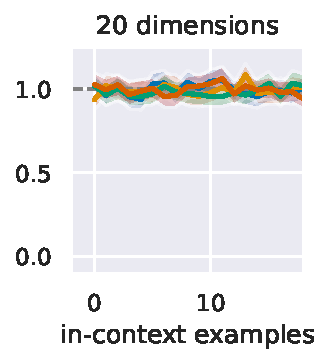
\includegraphics[height=.18\textwidth]{figures/trials/trial_orthogonal_20.pdf}
        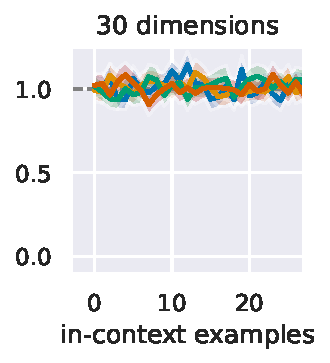
\includegraphics[height=.18\textwidth]{figures/trials/trial_orthogonal_30.pdf}
        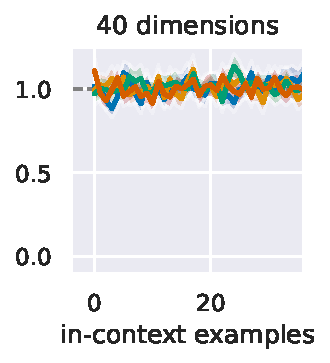
\includegraphics[height=.18\textwidth]{figures/trials/trial_orthogonal_40.pdf}
        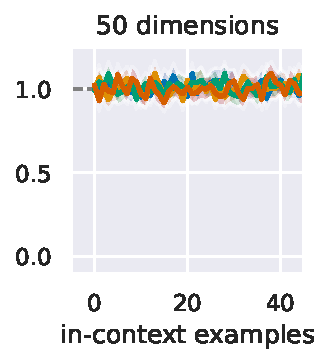
\includegraphics[height=.18\textwidth]{figures/trials/trial_orthogonal_50.pdf}
        \caption{orthogonal query}
        \label{fig:trial_orthogonal}
    \end{subfigure} \\[.7em]
    \begin{subfigure}[b]{\textwidth}
        \centering
        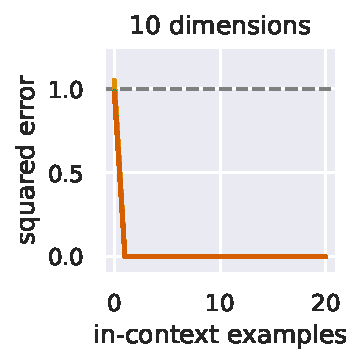
\includegraphics[height=.18\textwidth]{figures/trials/trial_overlapping_10.pdf}
        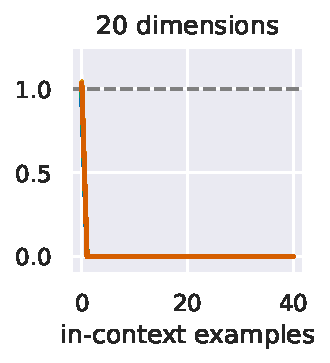
\includegraphics[height=.18\textwidth]{figures/trials/trial_overlapping_20.pdf}
        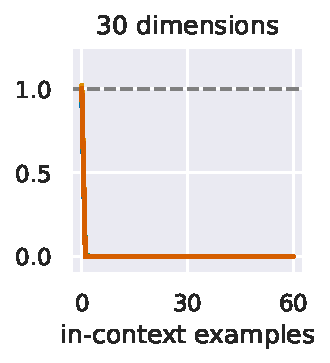
\includegraphics[height=.18\textwidth]{figures/trials/trial_overlapping_30.pdf}
        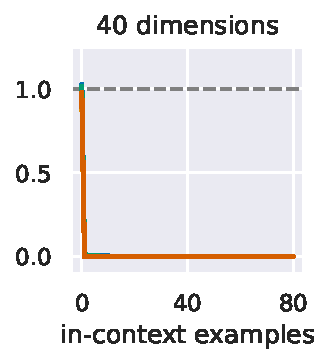
\includegraphics[height=.18\textwidth]{figures/trials/trial_overlapping_40.pdf}
        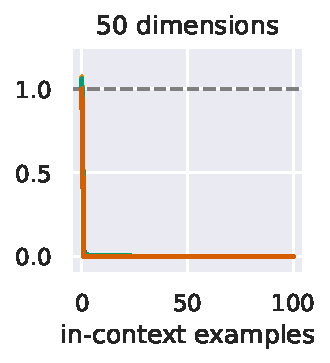
\includegraphics[height=.18\textwidth]{figures/trials/trial_overlapping_50.pdf}
        \caption{query matches in-context example}
        \label{fig:trial_overlapping}
    \end{subfigure} \\[.7em]
    \begin{subfigure}[b]{\textwidth}
        \centering
        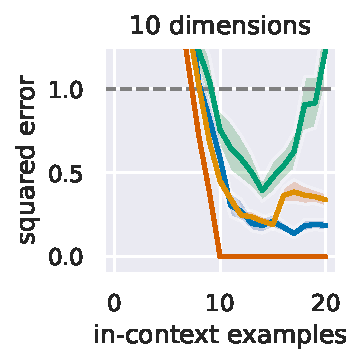
\includegraphics[height=.18\textwidth]{figures/trials/trial_scale-x=2_10.pdf}
        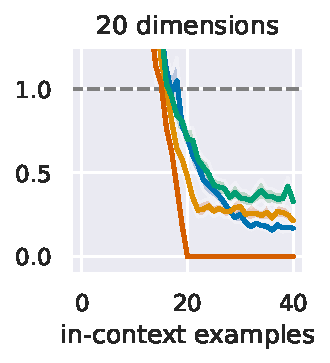
\includegraphics[height=.18\textwidth]{figures/trials/trial_scale-x=2_20.pdf}
        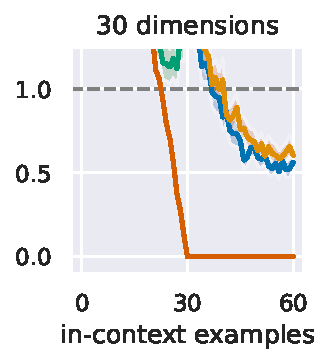
\includegraphics[height=.18\textwidth]{figures/trials/trial_scale-x=2_30.pdf}
        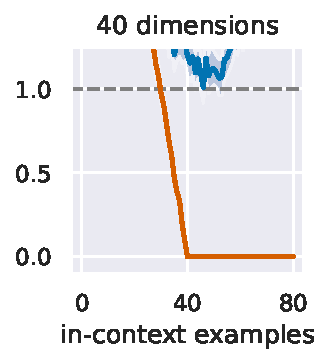
\includegraphics[height=.18\textwidth]{figures/trials/trial_scale-x=2_40.pdf}
        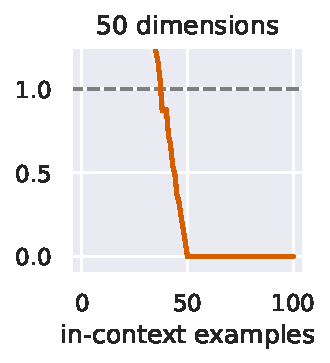
\includegraphics[height=.18\textwidth]{figures/trials/trial_scale-x=2_50.pdf}
        \caption{scaled $x$ by a factor of $2$}
        \label{fig:trial_scalex}
    \end{subfigure} \\[.7em]
    \begin{subfigure}[b]{\textwidth}
        \centering
        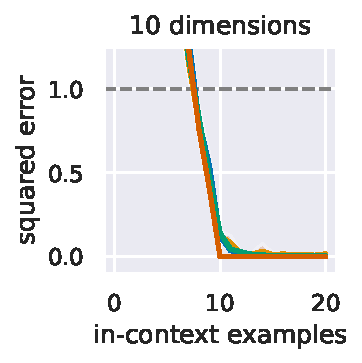
\includegraphics[height=.18\textwidth]{figures/trials/trial_scale-y=2_10.pdf}
        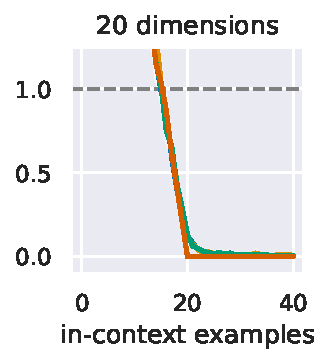
\includegraphics[height=.18\textwidth]{figures/trials/trial_scale-y=2_20.pdf}
        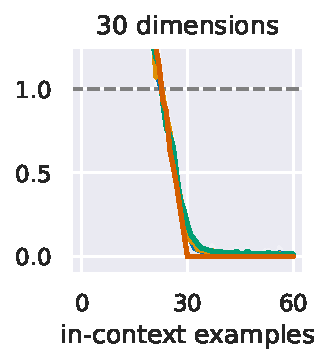
\includegraphics[height=.18\textwidth]{figures/trials/trial_scale-y=2_30.pdf}
        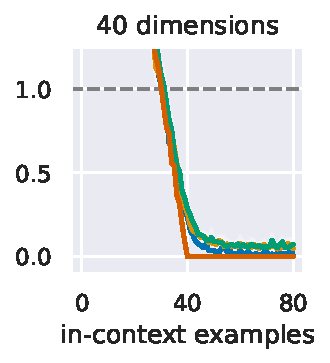
\includegraphics[height=.18\textwidth]{figures/trials/trial_scale-y=2_40.pdf}
        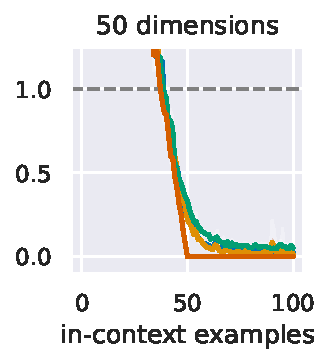
\includegraphics[height=.18\textwidth]{figures/trials/trial_scale-y=2_50.pdf}
        \caption{scaled $w$ by a factor of $2$}
        \label{fig:trial_scaley}
    \end{subfigure}
    \caption{(continued) \emph{Errors for models trained with different random seeds.} For each dimension, we train three models with different random seeds and show the corresponding error curves.}
    \label{fig:trials}
\end{figure}

\clearpage
\subsection{Curriculum}
\label{app:curriculum}
In Figure \ref{fig:curriculum}, we show the training loss of the Transformer model trained to in-context learn linear functions, with and without a curriculum. Specifically, given a random training prompt sequence $(x_1, f(x_1)$, $x_2, f(x_2)$, $\ldots$, $x_{k_\text{cur}}, f(x_{k_\text{cur}}))$, let $\hat{y_i}$ be the model's prediction for the $i^\text{th}$ input (meant to approximate $f(x_i)$). For each such prompt, we consider the loss given by the normalized squared error averaged over all prompt prefixes
\[
\frac{1}{k_{\text{cur}}}  \sum_{i=1}^{k_{\text{cur}}} 
\frac{\left(
\hat{y}_i - f(x_i)
\right)^2}{d}.
\]
At each training step, we plot the loss averaged over a batch of $64$ random prompts. For training with curriculum, $k_{\text{cur}}$ is gradually increased to $2d+1$  as described in Section \ref{app:training}. For training without curriculum $k_{\text{cur}} = 2d+1$ at all times. 

Note that the loss often increases in the beginning as we train the model with curriculum. This is due to a sharp increase in the loss at steps where we increase the effective dimensionality ($d_\text{cur}$) of prompt inputs ($x_i$). There are two reasons for this increase: (i) variance of the target output ($f(x_i) = w^\top x_i$) increases, so even the optimum loss is larger, (ii) the model performance is worse for the prompt inputs with increased effective dimension. After each such step where we increment $d_\text{cur}$, the loss starts to decrease again until the next increment. The overall trend in the loss looks upward when the sharp increase dominates the decrease that follows. Some observations worth highlighting are as follows.

\paragraph{Curriculum drastically speed-ups training.} For functions in 20 or more dimensions, curriculum allows us to train a low-error model often 4 times faster. Moreover, training without curriculum does not always succeed within our training budget (500k steps), e.g., for one run with $d=30$  and \emph{all} runs with $d=50$, the loss does not decrease at all without curriculum.
    
\paragraph{Initial lull without curriculum.}     For training without curriculum, we observe that the loss does not decrease for relatively a long period in the beginning, and starts to decrease sharply thereafter. There is a large variance in the length of this period for any fixed dimension, and  the average length  seems to increase with dimension. This period is almost non-existent for smaller dimensions (e.g., see the plot for $d=10$), and therefore we do not observe such a period while training with curriculum where we start training with inputs lying in a 5 dimensional subspace.



% For the 20 dimensional problem where we were able to train the model with and without curriculum, we did not observe any qualitative difference in model performance in the two settings. We show the corresponding plots for accuracy obtained with and without distribution shifts in Figure \ref{}.

\begin{figure}[htp]
    \centering
    \begin{subfigure}[b]{.32\textwidth}
        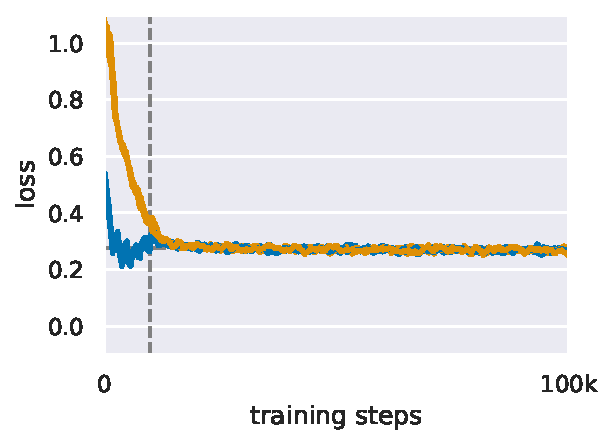
\includegraphics[height=.75\textwidth]{figures/curriculum_10.pdf}
        \caption{10 dimensions}
        \label{fig:curr_10}
    \end{subfigure}
    \begin{subfigure}[b]{.32\textwidth}
        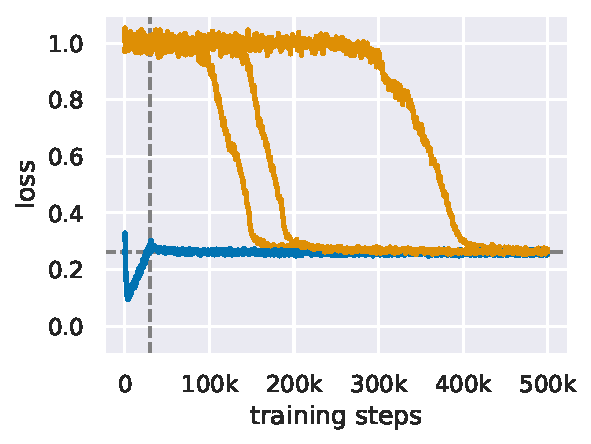
\includegraphics[height=.75\textwidth]{figures/curriculum_20.pdf}
        \caption{20 dimensions}
        \label{fig:curr_20}
    \end{subfigure}
    \begin{subfigure}[b]{.32\textwidth}
        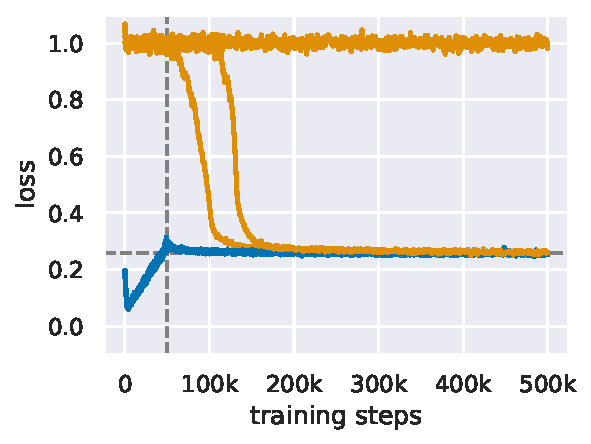
\includegraphics[height=.75\textwidth]{figures/curriculum_30.pdf}
        \caption{30 dimensions}
        \label{fig:curr_30}
    \end{subfigure}\\[1em]
    
    \begin{subfigure}[b]{.32\textwidth}
        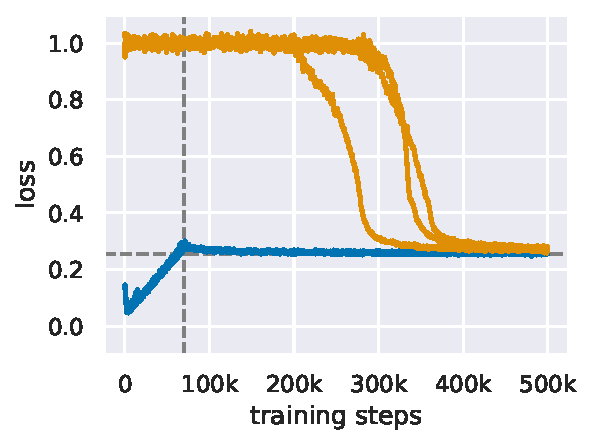
\includegraphics[height=.75\textwidth]{figures/curriculum_40.pdf}
        \caption{40 dimensions}
        \label{fig:curr_40}
    \end{subfigure}
    \begin{subfigure}[b]{.32\textwidth}
        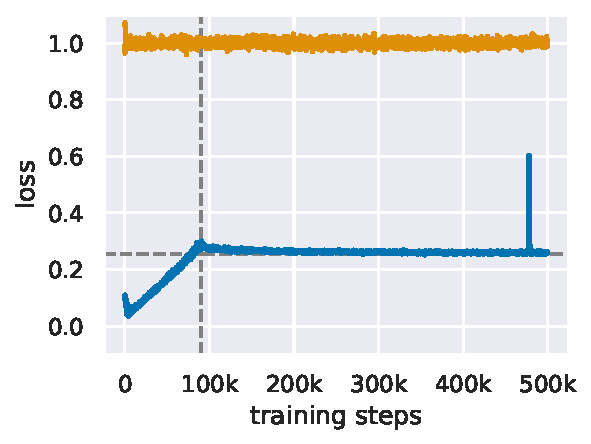
\includegraphics[height=.75\textwidth]{figures/curriculum_50.pdf}
        \caption{50 dimensions}
        \label{fig:curr_50}
    \end{subfigure}
    \begin{subfigure}[b]{.32\textwidth}
        \centering
        
\includegraphics[width=.8\textwidth]{figures/curriculum_legend.pdf}
        \vspace{2cm}
    \end{subfigure}
    \caption{\emph{Loss progression during training with and without curriculum.} For each dimension, we show the loss progression with 3 random seeds each for training with and without curriculum. The vertical dashed line shows the point at which the effective dimension of prompt inputs $d_\text{cur}$ reaches the actual dimension $d$, after which training with and without curriculum have the same prompt distribution. The horizontal dashed line shows the optimum expected loss.
    There is a drastic speedup in training with curriculum. Without curriculum, there is an initial relatively long period where the loss does not decrease. For each dimension, there is a large variance in the length of this period, and the average length seems to increase with dimension.
    }
    \label{fig:curriculum}
\end{figure}

\paragraph{Curriculum does not affect final performance significantly.} For our core setting  ($d=20$), where we are able to train the model to  low error even without curriculum, we do not observe any qualitative differences in the error in most cases (both with and without distribution shifts). One exception is the case with skewed covariance, where the model trained without curriculum seems to do slightly better. We plot the error curves for the standard, different orthants and skewed covariance cases in Figure \ref{fig:curr_ood}.

\begin{figure}[htp]
    \centering
    \begin{subfigure}[b]{.32\textwidth}
        \centering
        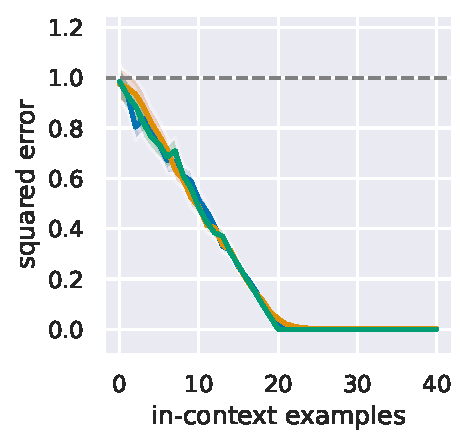
\includegraphics[height=.85\textwidth]{figures/curr_standard_20.pdf}
        \caption{standard}
    \end{subfigure}
    \begin{subfigure}[b]{.32\textwidth}
        \centering
        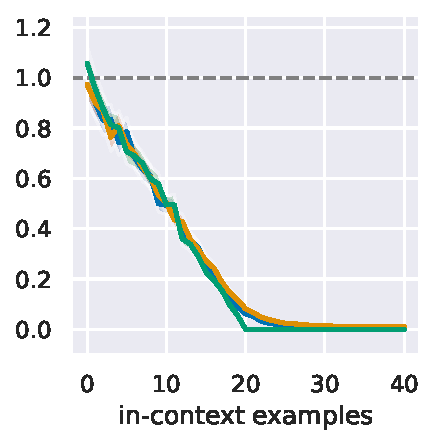
\includegraphics[height=.85\textwidth]{figures/curr_random_20.pdf}
        \caption{different orthants}
    \end{subfigure}
    \begin{subfigure}[b]{.32\textwidth}
        \centering
        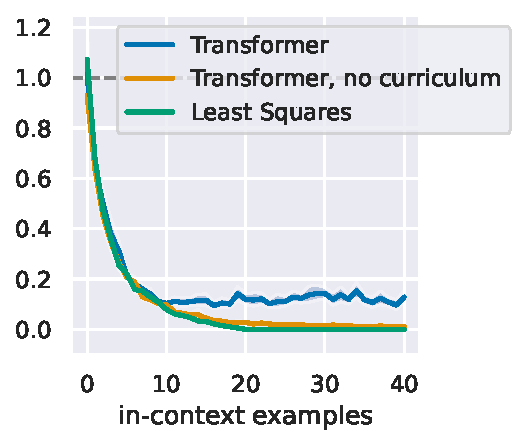
\includegraphics[height=.85\textwidth]{figures/curr_skewed_20.pdf}
        \caption{skewed}
    \end{subfigure}
    \caption{\emph{In-context learning performance for models trained with and without curriculum}. We show the  performance for models trained with and without curriculum for in-context learning linear functions ($d=20$). We did not observe any major qualitative difference in performance between the two settings in most cases. One exception is the case with skewed covariance where the model trained without curriculum does better. }
    \label{fig:curr_ood}
\end{figure}

\clearpage
\subsection{Effect of number of distinct prompts/functions seen during training}
\label{app:distinct_funcs}
Here, we investigate the effect of amount of training data required for in-context learning linear functions.

First, we consider the effect of number of distinct prompts encountered during training. For this, we create a set $S_p$ of $n_p$ randomly generated prompts, where each prompt in $S_p$ is generated by sampling a weight vector and prompt inputs from $N(0, I_d)$. We generate random prompts during training by sampling uniformly from this set. As before, we train the model for $500k$ steps with a batch size of $64$. We observe (see Figure \ref{fig:finite}) that a model trained with $n_p = 100k$ is able to achieve non-trivial error and a model trained with $n_p = 1M$ achieves error close to that of the unrestricted model (trained with $32M$ distinct prompts). Recall that with curriculum learning, we zero out some of the coordinates of prompt inputs in the beginning of training, which will increase the total number of prompts the model sees during training.
Therefore we do not use curriculum learning for this study to avoid inflating the number of distinct prompts seen during training. 



Second, we consider the effect of number of distinct weight vectors  (equivalently, distinct functions) encountered during training. For this, we create a set $S_w$ of $n_w$ weight vectors where each weight $w$ is drawn i.i.d. from $N(0, I_d)$. To generate a training prompt, $(x_1, w^\top x_1, \ldots, x_{k}, w^\top x_{k})$, we draw prompt inputs ($x_i$s) i.i.d. from $N(0, I_d)$ as in the unrestricted setting,  and sample $w$ uniformly at random from $S_w$. Thus while we sample from a finite set of weight vectors, we sample fresh inputs at each step. As before, we train the model for $500k$ steps with a batch size of $64$. Here, we observe (see Figure \ref{fig:finite}) that the model trained with as few as $10k$ distinct weight vectors achieves error close to the unrestricted model (trained with $32M$ distinct functions). We use curriculum learning for this study as in our standard setting. Recall that with curriculum learning, we only zero out some coordinates of prompt inputs in the beginning, so this does not change the number of distinct weight vectors seen by the model during training.
%We observe (see Figure \ref{fig:finite}) that even the model trained with $n_w = 100$ is able to achieve non-trivial error for large enough number of in-context examples. 
%Note that this is not trivial since the model cannot be memorizing individual $x_i$ values as these are sampled randomly and independently of $w$. 
% Moreover,  the model trained with $n_w = 10,000$ is able to achieve close to optimal error.

\begin{figure}[htp]
    \centering
    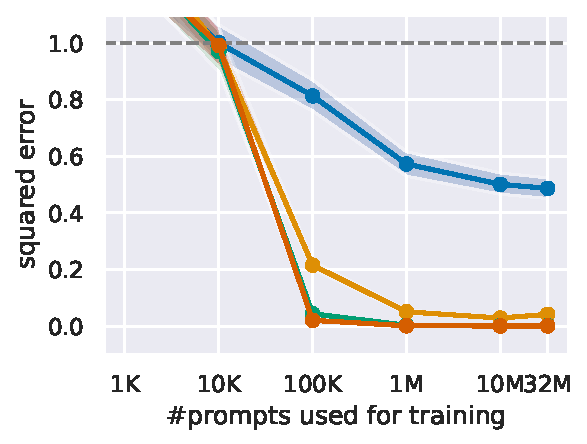
\includegraphics[height=.25\textwidth]{figures/examples.pdf}
    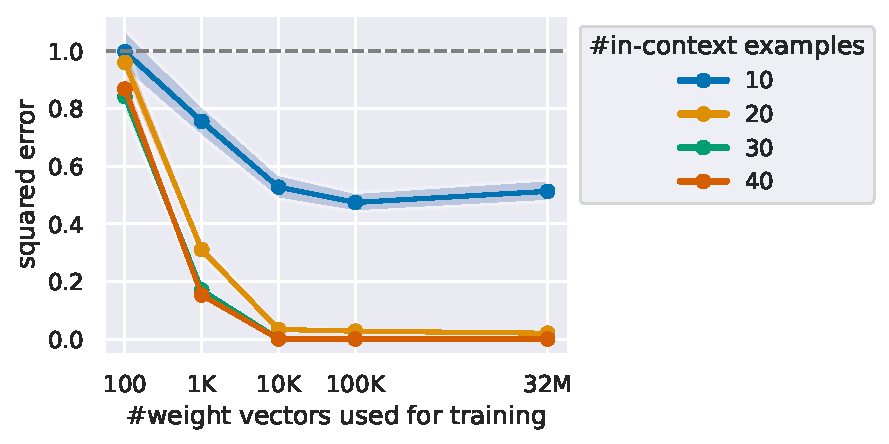
\includegraphics[height=.25\textwidth]{figures/finite.pdf}
    \caption{\emph{Effect of number of distinct prompts/functions seen during training.} We plot the squared error for models trained to in-context linear functions, as we increase the number of 
    distinct prompts and distinct weight vectors (equivalently, distinct functions) seen during training. (Note that 32M corresponds to the unrestricted model where we sample fresh prompts at each training step.) The models are able to achieve error close to that of the unrestricted model with  $1M$ distinct prompts or $10k$ distinct weight vectors.
    }
    \label{fig:finite}
\end{figure}

\clearpage
\subsection{Can memorization explain model performance?} 
\label{app:memorization}
In Section \ref{sec:linear_functions_1}, we discussed that memorization of prompts seen during training cannot explain model performance. 
This is because the probability of the model encountering a training prompt similar to the one used for testing is astronomically low---the prompt inputs alone lie in a 800-dimensional space when predicting with $2d$ in-context examples ($d=20$).

Moreover, even considering the possibility that the model encountered a similar \emph{weight vector} during training cannot explain its performance.
Let $S_w$ be the set of weight vectors used to generate training prompts. At inference time, given a prompt with in-context examples generated using a weight vector $w_\star$, suppose the model is somehow able to find the best weight vector $\hat{w}$ in $S_w$ minimizing the normalized squared error on query inputs:
\begin{align*}
\hat{w} &= \argmin_{w \in S_w} \ \mathds{E}_{x_{\text{query}} \sim N(0, I_d)} \left[\frac{(w^\top x_{\text{query}} - {w_\star}^\top x_{\text{query}}  )^2}{d} \right] \\
&= \argmin_{w \in S_w} \ \frac{ \lVert w - w* \rVert ^2_2}{d}
\end{align*}
Taking expectation over the weight vector $w_\star$, we get the expected normalized squared error of the model (with respect to randomly drawn in-context examples and query inputs):
\[
\mathds{E}_{{w_\star \sim N(0, I_d)}} \left[ \min_{w \in S_w} \ \frac{ \lVert w - w_\star \rVert ^2_2}{d} \right].
\]
To empirically estimate this quantity, we sample $n_w$ weight vectors from $N(0, I_d)$ (with $d = 20$) that form the set $S_w$, and $500$ weight vectors from $N(0, I_d)$ to estimate the outer expectation. We do this 20 times, freshly sampling the $500$ weight vectors and the vectors comprising $S_w$ each time, and compute the mean of the 20 estimates obtained. 
When $n_w = 32M$ (number of weight vectors encountered in our standard training setup), we get a mean of 0.216 (standard deviation 0.004). However, our model is able to achieve an expected error of less than $0.001$ for prompts with $2d$ in-context examples.
Similarly, when $n_w = 10,000$, we get a mean of 0.505 (standard deviation 0.006), while a model trained on prompts generated using $10,000$ distinct weight vectors is able to achieve a much smaller error (see Figure \ref{fig:finite}). 

Thus we can conclude that the model cannot be relying on memorization
of the training prompts or weight vectors, and is encoding a more sophisticated algorithm capable of in-context
learning linear functions that are very different from those seen during training.
